\documentclass[onecolumn]{article}
\raggedbottom

% === Idioma e codificação ===
\usepackage[utf8]{inputenc}
\usepackage[english]{babel}
\usepackage[T1]{fontenc}

% === Pacotes matemáticos e símbolos ===
\usepackage{amsmath, amssymb, amsfonts}

% === Figuras e gráficos ===
\usepackage{graphicx}
\usepackage{float}        % para [H]
\usepackage{adjustbox}

% === Tabelas ===
\usepackage{booktabs}     % \toprule etc.
\usepackage{multirow}
\usepackage{array}
\usepackage{makecell}
\usepackage{tabularx}
\usepackage{siunitx}      % unidades físicas
\usepackage{longtable}


% === Estilo e layout ===
\usepackage[font=small]{caption}  % Apenas uma chamada do pacote 'caption'
\usepackage{titlesec}
\usepackage{geometry}
\usepackage{indentfirst}
\usepackage{balance}
\usepackage{blindtext}
\usepackage{titlesec}

% === Código fonte (C++, Python, etc.) ===
\usepackage{listings}
\usepackage{xcolor}
\lstset{
  basicstyle=\ttfamily\small,
  frame=single,
  breaklines=true,
  columns=fullflexible,
  numbers=none  % ← disables line numbers
}

% === Extras ===
\usepackage{isotope}
\usepackage{hyperref}
\usepackage{tcolorbox}

% === Notas de rodapé em figuras/tabelas ===
\usepackage{footnote}
\makesavenoteenv{figure}
\makesavenoteenv{table}



\lstset{
  language=C++,
  basicstyle=\ttfamily\footnotesize,
  keywordstyle=\color{blue},
  commentstyle=\color{gray},
  stringstyle=\color{orange},
  numbers=left,
  numberstyle=\tiny,
  stepnumber=1,
  numbersep=10pt,
  backgroundcolor=\color{white},
  frame=single,
  breaklines=true,
  breakatwhitespace=false,
  tabsize=2,
  captionpos=b
}

% === Títulos menores e centrados ===
\titleformat{\section}{\normalfont\Large\centering}{\thesection}{1em}{}
\titleformat{\subsection}{\normalfont\large}{\thesubsection}{1em}{}

% === Evita espaços verticais gigantes nas colunas ===
\raggedbottom

% === Título ===
\title{
    PPS Cold Box - RaspberryPi setup\\
   
}
\author{
José Miguel\\
}
\date{July 2025}


%-%-%-%-%-%-%-%-%-%-%- M A R G I N S -%-%-%-%-%-%-%-%-%-%-%
\geometry{  a4paper,
            left=1.5 cm,
            top=2 cm,
            right=1.5 cm,
            bottom=1.5 cm}   


\begin{document}

\maketitle

\tableofcontents

\newpage
\normalsize




\section{Introduction}
    This pdf is part of a folder containing other files; those files will come in handy throughout the tutorial. Please make sure to update the Raspberry Pi and have everything up to date with:
    

\begin{lstlisting}[numbers=none]
    sudo apt update
    sudo apt upgrade
\end{lstlisting}

    SSH should be enabled, and a static IP address is required. Furthermore, make sure that $I^2C$ communication is enabled. Use "sudo raspi-config" and navigate to "Interfaces Options" -> "I2C". \\

    Install all the necessary packages:

\begin{lstlisting}[numbers=none]
sudo apt install -y python3-pip python3-smbus python3-rpi.gpio python3-gpiozero \
i2c-tools python3-smbus2 python3-paho-mqtt python3-scipy
\end{lstlisting}
    

\section{Server and Data Visualization}

\subsection{Setting up Docker}
To start the installation process, download IoTStack using the following command, it should reboot once the download is complete:

\begin{lstlisting}[
    keywordstyle=\color{black},
    commentstyle=\color{black},
    stringstyle=\color{black},
    numbers=none]
    curl -fsSL https://raw.githubusercontent.com/SensorsIot/IOTstack/master/install.sh | bash
\end{lstlisting}

If any prompt shows up to download certain packages, do accept. Once the Pi is back, navigate to the IoTStack folder, then run the menu script:

\begin{lstlisting}[numbers=none]
    cd IOTstack/
    ./menu.sh
\end{lstlisting}

Use enter to select "Build Stack". Use the "up" and "down" arrows to navigate between packages. Press the space bar to select: Grafana, Influxdb, Mosquitto and NodeRed. The interface can glitch quite a bit, make sure to use the fullscreen mode. Furthermore, there are two Influxdb options; select Influxdb, not Influxdb2.

There will be a warning message upon selecting the NodeRed package, simply press the right arrow key to enter the options menu, hit "Select \& build addons list" and accept the default. Navigate back to the packages menu.\\

Press "Enter" to begin build, navigate to "Docker commands" and select "Start stack"

After the setup is finished, run the command:

\begin{lstlisting}[numbers=none]
    docker-compose ps
\end{lstlisting}

The output should be something like the following (Created and Status columns adjusted to when the containers were created):

\scriptsize
\begin{longtable}{@{}>{\raggedright\arraybackslash}p{2cm}%
                    >{\raggedright\arraybackslash}p{2.5cm}%
                    >{\raggedright\arraybackslash}p{3.5cm}%
                    >{\raggedright\arraybackslash}p{2cm}%
                    >{\raggedright\arraybackslash}p{2cm}%
                    >{\raggedright\arraybackslash}p{3.5cm}@{}}
\toprule
\textbf{Service} & \textbf{Image} & \textbf{Command} & \textbf{Created} & \textbf{Status} & \textbf{Ports} \\
\midrule
grafana        & grafana/grafana         & \texttt{/run.sh}                        & 2 days ago & Up 20 hours (healthy) & 0.0.0.0:3000$\rightarrow$3000/tcp, [::]:3000$\rightarrow$3000/tcp \\
influxdb       & influxdb:1.8            & \texttt{/entrypoint.sh influxd}         & 5 days ago & Up 20 hours (healthy) & 0.0.0.0:8086$\rightarrow$8086/tcp, [::]:8086$\rightarrow$8886/tcp \\
mosquitto      & iotstack-mosquitto      & \texttt{/docker-entrypoint.sh}         & 5 days ago & Up 20 hours (healthy) & 0.0.0.0:1883$\rightarrow$1883/tcp, [::]:1883$\rightarrow$1883/tcp \\
nodered        & iotstack-nodered        & \texttt{./entrypoint.sh}               & 5 days ago & Up 20 hours (healthy) & 0.0.0.0:1880$\rightarrow$1880/tcp, [::]:1889$\rightarrow$1880/tcp \\
\bottomrule
\end{longtable}

\subsection{Setting up Influxdb}
\normalsize

Inside the IOTstack folder, run the following command to enter the INfluxDB container:

\begin{lstlisting}[numbers=none]
    docker exec -it influxdb influx
\end{lstlisting}

Create a database named "sensor\_data" and exit using:

\begin{lstlisting}[numbers=none]
    CREATE DATABASE sensor_data
    quit

\end{lstlisting}

\subsection{Setting up Node-Red}
    Open Node-Red using a Web browser. If the set-up is being done via the Raspberry Pi, search: 

    \begin{lstlisting}[
    keywordstyle=\color{black},
    commentstyle=\color{black},
    stringstyle=\color{black},
    numbers=none]
        http://localhost:1880
    \end{lstlisting}

    Otherwise, use:

    \begin{lstlisting}[
    keywordstyle=\color{black},
    commentstyle=\color{black},
    stringstyle=\color{black},
    numbers=none]
        http://<ip_address>:1880
    \end{lstlisting}

    Open the drop-down menu in the top right corner and select "Import". Click "Select a file to import" and import the file "flows.json" from the provided folder. A new flow should have been created. It should look something like this:
    
\begin{figure}[H]
    \centering
    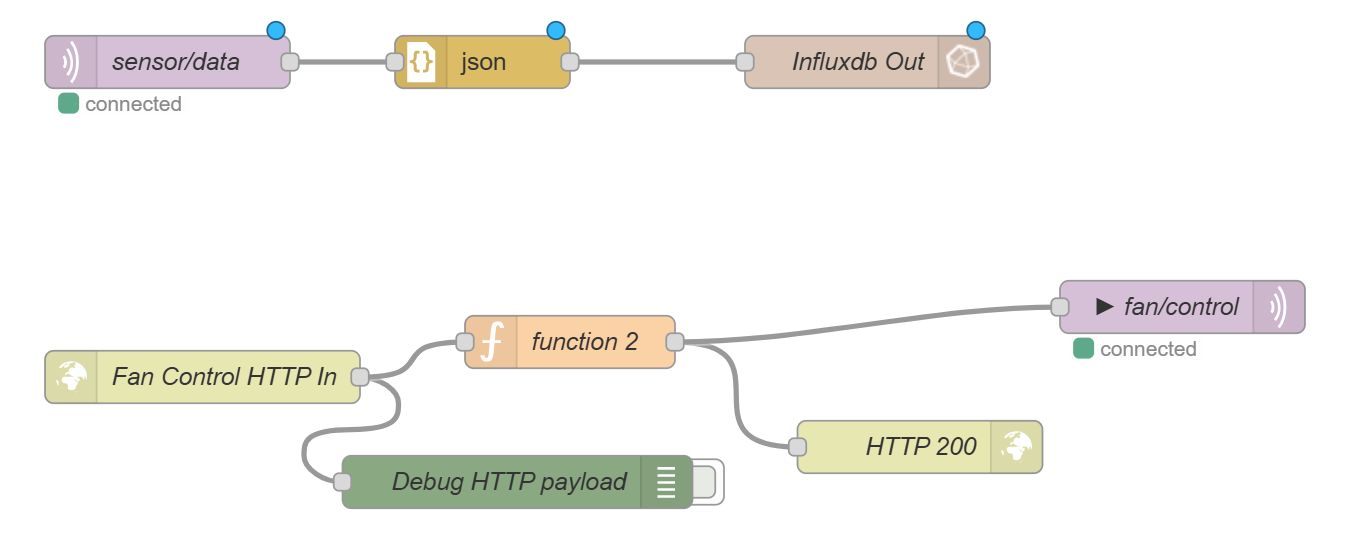
\includegraphics[width=0.5\textwidth]{nodered.png}
    \caption{Node-Red flow configuration}
    \label{fig:NodeRed} 
\end{figure}

    Before hitting "Deploy", double click each node to edit. Make sure of the following:


\subsubsection*{MQTT In Node: \texttt{sensor/data}}

\begin{itemize}
  \item \textbf{Server:} MQTT Docker 
  \begin{itemize}
      \item \textbf{Name:} MQTT Docker
      \item \textcolor{red}{\textbf{Server:}} \texttt{<ip\_address>}  \textbf{Port:} 1883
      \item \textbf{Connect Automatically}
      \item \textbf{Protocol:} MQTT V3.1.1
  \end{itemize}
  \item \textcolor{red}{\textbf{Topic:}} \texttt{sensor/data}
  \item \textbf{Output format:} a parsed JSON object
  
\end{itemize}

\subsubsection*{JSON Node}

\begin{itemize}
  \item \textbf{Action:} Always convert to JavaScript object
  \item \textbf{Property:} msg. payload
\end{itemize}

\subsubsection*{InfluxDB Out Node}

\begin{itemize}
  \item \textbf{Measurement:} \texttt{environment}
  \item \textbf{Server:}
    \begin{itemize}
      \item \textcolor{red}{\textbf{Database:}} \texttt{sensor\_data}
      \item \textbf{InfluxDB Version:} 1.x
      \item \textcolor{red}{\textbf{Host:}} \texttt{<ip\_address>}
      \item \textbf{Port:} 8086
    \end{itemize}
\end{itemize}

\subsubsection*{HTTP In Node: \texttt{/fan}}

\begin{itemize}
  \item \textbf{Method:} GET
  \item \textbf{URL:} \texttt{/fan}
\end{itemize}

\subsubsection*{Function Node:}

\begin{itemize}
  \item \textbf{On Message:}
\end{itemize}

\begin{lstlisting}[numbers=none]
        // msg.req.query.duty contains the numeric duty from the URL
        const duty = parseInt(msg.req.query.duty, 10);
        if (!isNaN(duty) && duty >= 0 && duty <= 100) {
           msg.payload = duty;
        } else {
            node.error("Invalid duty: " + msg.req.query.duty);
            msg.payload = 0;
        }
        return msg;
\end{lstlisting}

\subsubsection*{HTTP Response Node:}

\begin{itemize}
  \item \textbf{Status Code:} 200
\end{itemize}

\subsubsection*{MQTT Out Node:}

\begin{itemize}
  \item \textbf{Server:} Mosquitto
  \begin{itemize}
      \item \textbf{Name:} Mosquitto
      \item \textcolor{red}{\textbf{Server:}} \texttt{mosquitto}  \textbf{Port:} 1883
      \item \textbf{Connect Automatically}
      \item \textbf{Protocol:} MQTT V3.1.1
  \end{itemize}
  \item \textbf{Topic:} \texttt{fan/control}
  \item \textbf{QoS:} 0
\end{itemize}

\vspace{1cm}

\textbf{Hit "Deploy", the MQTT in and out nodes should go from red: Disconnected to green: Connected in a few seconds.}

\subsubsection{Debugging:}

Return to the Raspberry Pi terminal, navigate to the IOTstack folder, and run the following list of commands to check that data are being written to the database:
\label{influxdebug}

\begin{lstlisting}[numbers=none]
    docker exec -it influxdb influx
    USE sensor_data
    show measurements
    select * from environment
    quit
\end{lstlisting}

If nothing shows, it means that the data is not reaching Influxdb. Run the following command to subscribe to the MQTT topic and receive the transmitted data:


\begin{lstlisting}[numbers=none]
    docker exec -it mosquitto mosquitto_sub -v -t /sensor/data
\end{lstlisting}

If data appears, then the error is most likely due to node red. Start by checking the servers and the debug terminal (the third of the four square-button menu just below deploy) to identify the node at fault. Feel free to add a debug node to better visualize the issue.


\subsection{Setting up Grafana}
When entering Grafana for the first time, the username and password are "admin". Then it will prompt you to change the password. 

\subsubsection{Adding a Database}
On the main menu, under "Welcome to Grafana", click "Add your first data source". Select Influxdb.

Under "HTTP", type the url:

\begin{lstlisting}[
    keywordstyle=\color{black},
    commentstyle=\color{black},
    stringstyle=\color{black},
    numbers=none]
    http://<ip_address>:8086
\end{lstlisting}

Under InfluxDB Details, set the following:

\begin{itemize}
    \item \textbf{Database:} \texttt{sensor\_data}
    \item \textbf{HTTP Method:} GET
    \item \textbf{Min time interval:} 1s
    \item \textbf{Max series:} Choose accordingly
\end{itemize}

Click "Save \& test", you should see the following message:

\begin{tcolorbox}[colback=white,colframe=black!100, arc=0mm, boxrule=0.4pt]
     datasource is working. 1 measurements found \\
Next, you can start to visualize data by \underline{building a dashboard}, or by querying data in the \underline{Explore view}.
\end{tcolorbox}

Select "building a dashboard".

\subsubsection{Building a Dashboard}
\normalsize
Click "Import a Dashboard", discard the current one, and import the JSON file named "Fan\&Monitor".\\

To modify the dashboard, enter edit mode, drag the panels and change their sizes. To edit a specific panel, click the three dots and "Edit". The only relevant settings are the "Visualization" type (eg. Time Series vs Gauge), the Data Source (InfluxDB), the FROM (Default \& "environment") and the SELECT field to select the dependent variable. Everything else is more a matter of aesthetics. \\

To control the fan, the panel should have the visualization type "Text", be in Markdown mode and the content should be the following (make sure to update the \textcolor{red}{ip address}): \\

\begin{lstlisting}[
    keywordstyle=\color{black},
    commentstyle=\color{black},
    stringstyle=\color{black},
    numbers=none]
### Fan Control 
[Fan Off](http://<ip_address>:1880/fan?duty=0)  
[Fan 25%](http://<ip_address>:1880/fan?duty=25) 
[Fan 50%](http://<ip_address>:1880/fan?duty=50) 
[Fan 75%](http://<ip_address>:1880/fan?duty=75) 
[Fan 100%](http://<ip_address>:1880/fan?duty=100)
\end{lstlisting}

\subsubsection{Debugging:}
Make sure that the data source is configured correctly and contains data for Grafana to read (refer back to \ref{influxdebug}). A not-very-common bug is the uid of the influxdb datasource, which causes all panels to show a warning sign (this is accessable by opening the menu of any panel, hitting "Inspect" and selecting "Panel JSON"). The solution is to edit each panel individually and refresh it. 
   



\section{Adjustments to the main script}

The only things that might need adjustment are the ADC channels being read and the interval between data acquisitions. For the latter, simply change the variable SAMPLE\_INTERVAL at the top of the script. To adjust the ADC channels, look for the initialization of the ADC128D818 class within the sensor\_loop() function and change the list of channels (0-7):

\begin{lstlisting}[
    keywordstyle=\color{black},
    commentstyle=\color{black},
    stringstyle=\color{black},
    language=python,
    numbers=none]
    def sensor_loop():
        
        #Thread target: read sensors at fixed intervals,
        #build JSON payload, and publish via MQTT.
        
        sensor = BME280()
        adc    = ADC128D818(channels=(6, 7))
        next_time = time.time()
        bme_errors = 0

    (...)
\end{lstlisting}

Nevertheless, the script has a nice amount of commenting to allow the user to understand and adapt it as they see fit.\\

\textbf{NOTE:} Everytime the script is updated after the implementation of the Daemon (next section) the latter should be updated by running:

\begin{lstlisting}[numbers=none]
sudo systemctl daemon-reload
sudo systemctl start fanmonitor
\end{lstlisting}

\newpage

\section{Setting up the Daemon}

Saved a unit file using [test] 

\begin{lstlisting}[numbers=none]
    sudo nano /etc/systemd/system/fanmonitor.service
\end{lstlisting}
    
with the following content:\\


\begin{lstlisting}[numbers=none]
[Unit]
Description=Fan Monitor Script
After=network.target

[Service]
ExecStart=/usr/bin/python3 /home/pi/pps_cold_box.py
WorkingDirectory=/home/pi
StandardOutput=inherit
StandardError=inherit
Restart=always
User=pi

[Install]
WantedBy=multi-user.target
\end{lstlisting}

Adjust the following settings if need be:\\
\small

\textbf{ExecStart:} Full path to the Python interpreter and then to the script.

\textbf{User=pi \& Working Directory:} Run under the pi user

\normalsize

Reload, Enable, and Start the Service:
\begin{lstlisting}[numbers=none]
sudo systemctl daemon-reload
sudo systemctl enable fanmonitor
sudo systemctl start fanmonitor
\end{lstlisting}

Check that it is \textcolor{green}{active (running)}:

\begin{lstlisting}[numbers=none]
    sudo systemctl status fanmonitor
\end{lstlisting}


Tail live logs to ensure sensor publishes and fan-control messages are received:

\begin{lstlisting}[numbers=none]
    sudo journalctl -u fanmonitor -f
\end{lstlisting}

\section{Access Influxdb as a pandas dataframe}
A secondary script titled "influx\_reader.py" was also created as an option to facilitate the extraction and analysis of data. It was created to be versatile; depending on the data and data that need to be extracted, as well as its format. To use it, install the following packages:

\begin{lstlisting}[numbers=none]
    sudo apt install python3-pandas
    sudo apt install python3-influxdb
    sudo apt install python3-tabulate
    sudo apt install python3-pyarrow
\end{lstlisting}

By default, the program prints a table with the data requested, but there are options to select JSON, CSV or Feather formats, simply adjust the user configuration at the beginning of the sript:
\begin{lstlisting}[numbers=none, language=python]
    # -- USER CONFIG --------------------------------------- 
HOST           = "localhost"
PORT           = 8086
DATABASE       = "sensor_data"
MEASUREMENT    = "environment"

EXPORT_CSV     = False    #  set True to extract as CSV
EXPORT_JSON    = False    #  set True to extract as JSON
EXPORT_FEATHER = False    #  set True to extract as Feather

CSV_OUTFILE    = "output.csv"
JSON_OUTFILE   = "output.json"
FEATHER_OUTFILE= "output.feather"
    #--------------------------------------------------------
\end{lstlisting}

It is also quite straightforward to adjust the type of data extracted by changing the influx query, for example:

\begin{lstlisting}[numbers=none]
    # Connect & fetch
    client = InfluxDBClient(host=HOST, port=PORT, database=DATABASE)
    
    q = (
       f'SELECT time, temperature, humidity FROM "{MEASUREMENT}" '
       f"WHERE time >= '{start}' AND time <= '{end}'"
    )
    
\end{lstlisting}




\balance  % balance the columns for a cleaner layout

\vspace{1ex}
\noindent\hspace*{\fill}\rule{0.33\textwidth}{0.6pt}\hspace*{\fill}
\vspace{1ex}


\addcontentsline{toc}{section}{References \& Datasheets}

\small
\begin{thebibliography}{10}


\bibitem{BME280-Datasheet}
Bosch \ Sensortec GmbH. (2024). \emph{BME280 Data sheet} (Document revision\ 1.24, BST‑BME280‑DS001‑24). Retrieved July\ 16,\ 2025, from \url{https://www.bosch-sensortec.com/media/boschsensortec/downloads/datasheets/bme280/BST-BME280-DS001-24.pdf}

\bibitem{ADC128D818-Datasheet}
Texas \ Instruments Inc. (2015). \emph{ADC128D818 12‑Bit, 8‑Channel, ADC System Monitor With Temperature Sensor, Internal–External Reference, and I2C Interface} (SNAS483F–FEBRUARY\ 2010–REVISED\ AUGUST\ 2015). Retrieved July\ 16,\ 2025, from \url{https://www.ti.com/product/ADC128D818}

\bibitem{PTFD102A1A0-Datasheet}
TE\ Connectivity Measurement Specialties. (2020). \emph{PTFD102A1A0 PT1000,\ 2.0\ × 5.0\ A Industrial Temperature Sensor} (Version\ 2\ 10/2020). Retrieved July\ 16,\ 2025, from \url{https://pt.mouser.com/ProductDetail/Measurement-Specialties/PTFD102A1A0?qs=bvCpHSZmQjl6myCYnXHj%2FA%3D%3D}



\end{thebibliography}

\newpage
\appendix

\vspace{-2em}

\end{document}
